\section{Potenciais de medida conhecida}

Podemos validar a execução do programa e qualidade da medida gerada utilizando de potenciais bem descritos na literatura. Para isso, retomaremos os resultados da Seção \ref{Section: Potencias}. Foi comentado que modelos de matrizes aleatórias são úteis em simulações das medidas quando um modelo está disponível. A família de ensembles gaussianos são modelos que mostramos ser bem representados como matrizes em \ref{Section: Ensembles Gaussianos}. Note que tomar esta família é o equivalente, na simulação descrita a tomar os parâmetros 
\begin{equation}
d = 1, \ \  n = 2, \ \ \V(x)=\frac{|x|^2}{2}, \ \ W(x) = g(x) = \log{|x|}, \ \ \beta_N = \beta N^2, \ \ \beta = 1,2,4.
\label{Equation: Parametros Gaussian}
\end{equation}
Para demonstrar esta fato e representar a semelhança entra os dois métodos de simulação apresenta-se, para $N=10$, sem muitos detalhes da implementação, a densidade gerada para os três modelos ($\beta = 1,2,4$) na coluna da esquerda da Figura \ref{Figura: Gaussian}. Na mesma figura, também apresentamos a representação do Semi-Círculo de Wigner e o comportamento da configuração de equilíbrio para os três modelos quando $N$ cresce. Fica fácil observar a convergência para a medida de equilíbrio prevista. Note que os valores foram escalados por $\sqrt{2\beta}$ para melhor visualização.
\begin{figure}[ht]
	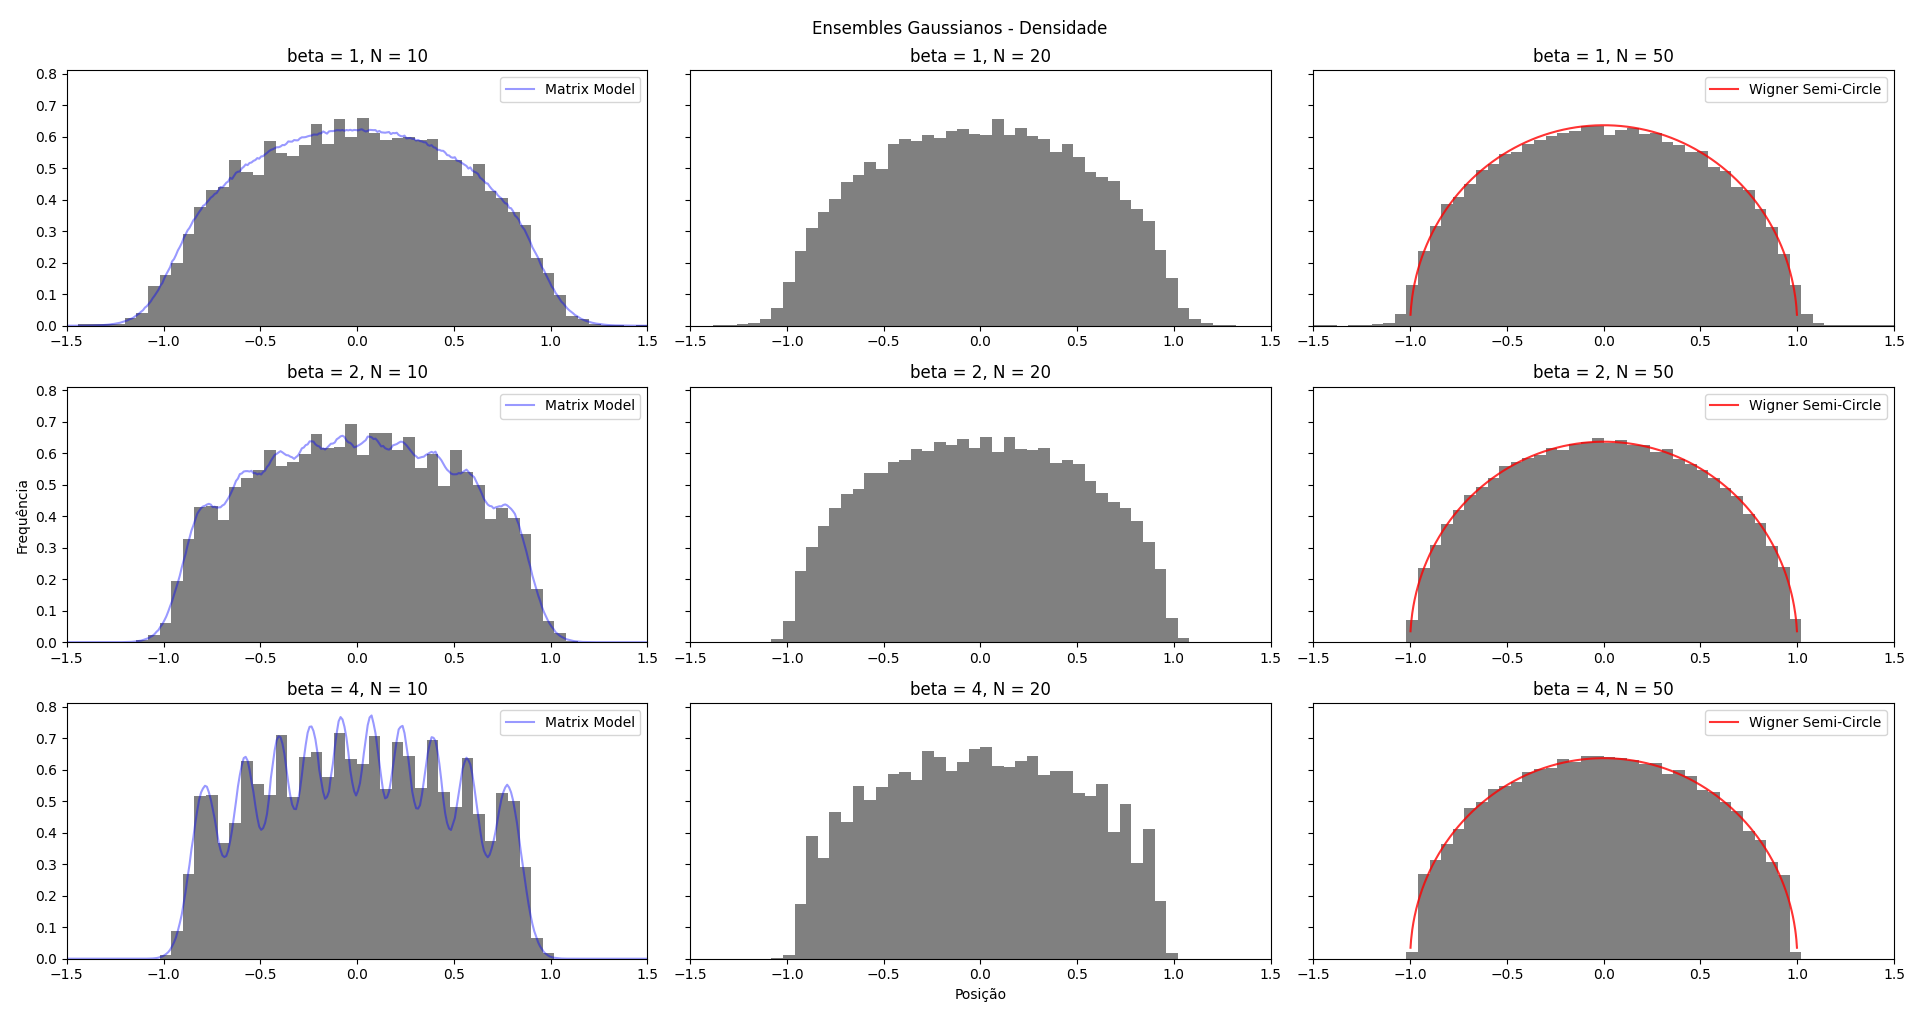
\includegraphics[width=\textwidth]{Assets/validationGaussian.png}
	\caption{Medidas de equilíbrio para os ensembles gaussianos, equivalente à tomar \ref{Equation: Parametros Gaussian}. Para todos, vale a escolha de $\Delta t = 0.5$ e $nsteps = 2\cdot10^6$ passos, registrando a cada $1000$ iterações os microestados a partir da metade da simulação. Para as simulações à esquerda da figura se apresenta ainda a distribuição da amostragem de $10^6$ matrizes do tipo apropriado e a densidade resultante.}
	\label{Figura: Gaussian}
\end{figure}

Indo além dos modelos gaussianos podemos retomar as descrições dos potenciais Mônico em \ref{Equação: Mônico} e as duas situações para o potencial quártico \ref{Equação: Quartico +} e \ref{Equação: Quartico -}. Respectivamente, estes modelos equivalem a tomar na simulação os parâmetros
\begin{equation}
	d = 1, \ \  n = 2, \ \ \V(x)= t |x|^{2m}, \ \ W(x) = g(x) = \log{|x|}, \ \ \beta_N = \beta N^2, \ \ \beta = 2.
	\label{Equation: Parametros Monico}
\end{equation}
\begin{equation}
	d = 1, \ \  n = 2, \ \ \V(x)=\frac{|x|^4}{4} + t \frac{|x|^2}{2}, \ \ W(x) = g(x) = \log{|x|}, \ \ \beta_N = \beta N^2, \ \ \beta = 2.
	\label{Equation: Parametros Quartico}
\end{equation}
Note que o caso mônico se reduz ao gaussiano se tomarmos $m=1$. Isso pode ser confirmado na figura \ref{Figura: Quartic Monic} onde a medida do semi-círculo é concordante com a simulação.
\begin{figure}[ht]
	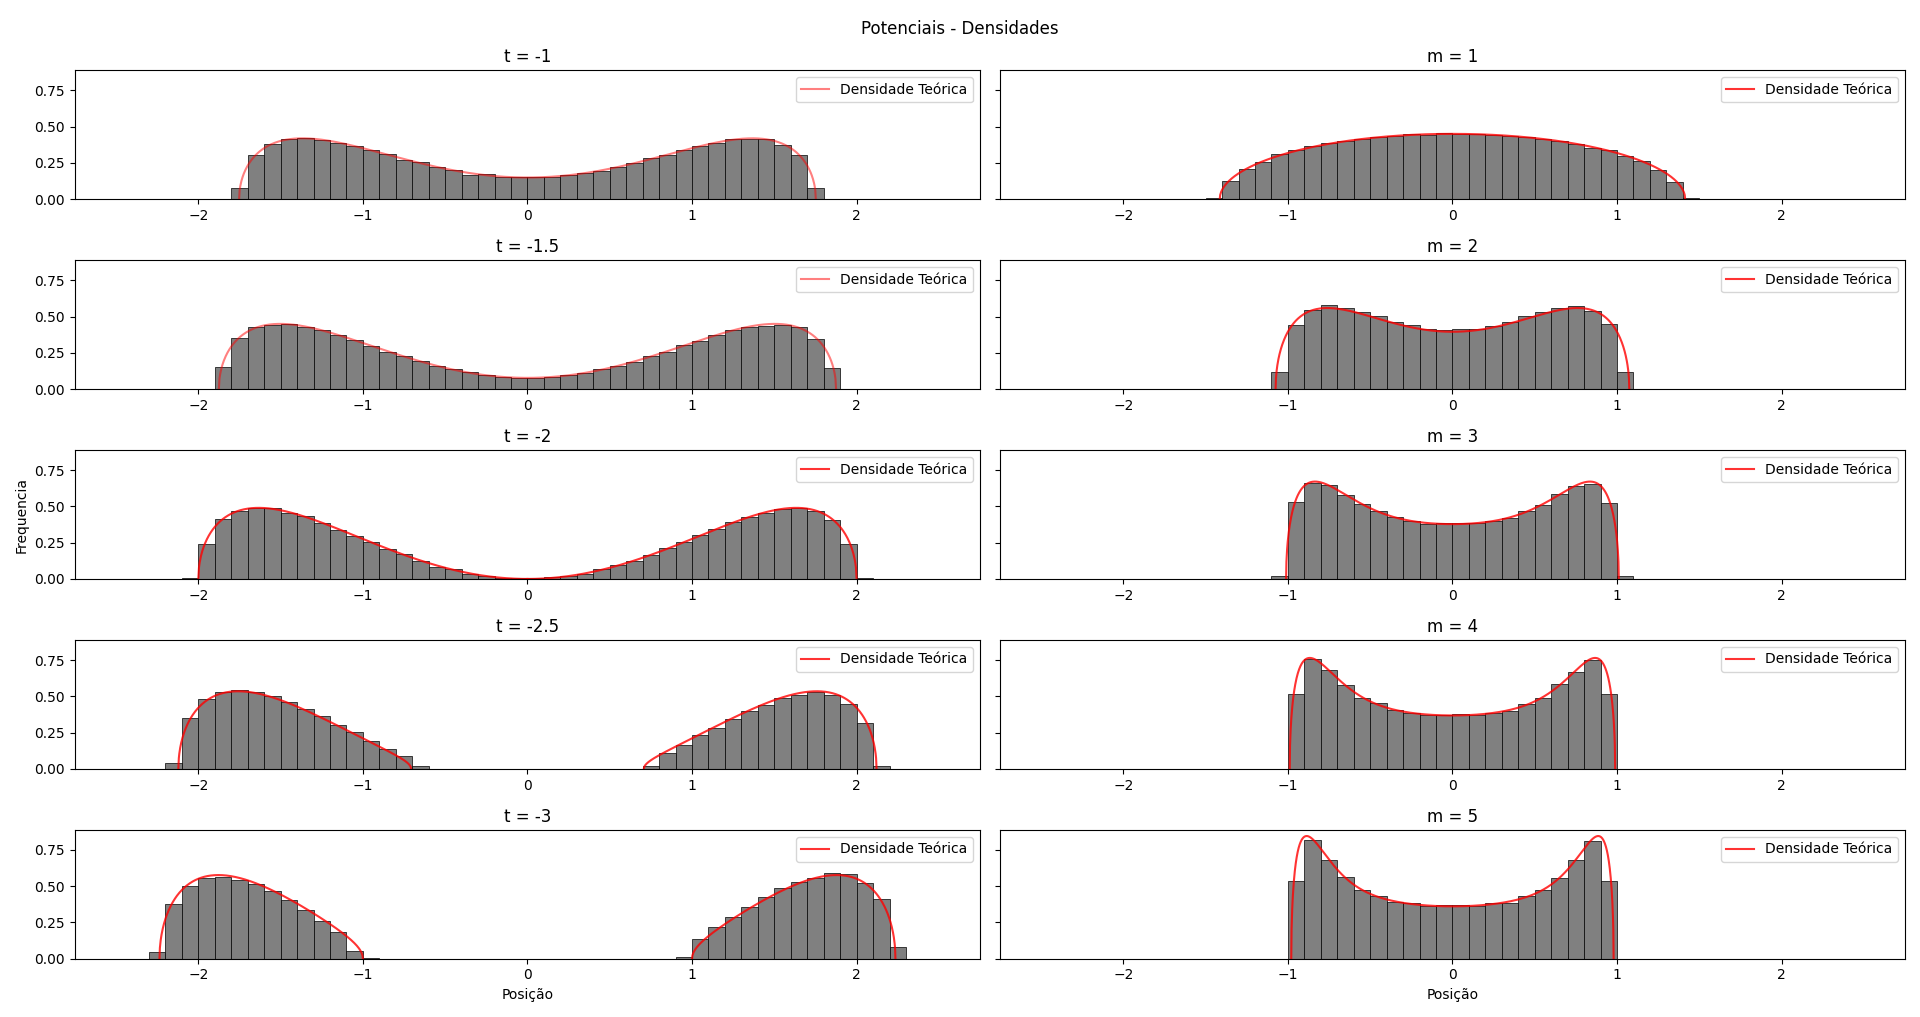
\includegraphics[width=\textwidth]{Assets/validationQuarticMonic.png}
	\caption{Medidas de equilíbrio para os potencias Quártico \ref{Equation: Parametros Quartico} e Mônico \ref{Equation: Parametros Monico}, respectivamente à esquerda e direita. Para ambos os casos vale $\Delta t = 0.5$ e $nsteps = 2\cdot10^6$ passos. Registra-se a cada $1000$ iterações os microestados a partir da metade da simulação. Toma-se por padrão $N=50$. No quártico, simula-se $t=-1,-1.5,-2,-2.5,-3$ e par ao mônico fixa-se $t=1$ e simula-se $m=1,2,3,4,5$.}
	\label{Figura: Quartic Monic}
\end{figure}
